\section{Fiducial Cuts}

\subsection{Introduction}

Similarly to the electron case, a fiducial cut on protons is introduced to constrain regions of phase space
where the CLAS response peaks at its maximum and remains rather smooth.
Detector inefficiencies not perfectly reproduced with GSIM are removed with dedicated cuts.

The fiducial regions were traditionally defined in the lab coordinates of the proton reconstructed $\phi, \theta, p$.
As for the electrons, it is more natural to define the fiducial regions in the detector coordinates, because
the inefficiencies are caused by tracks near their borders or hardware problems. Since the original approach
has been used in several published CLAS papers, we will include it in this note
as a reference.

\subsection{Traditional cuts on the electron lab coordinates $\phi, \theta, p$}
The fiducial cut in the lab coordinates has been determined during the $\pi^0$ analysis in
the $\Delta(1232)$ region \cite{bib:pi0_Delta}.

Unlike the electron case, the $\phi$ boundaries are asymmetric, as shown in
Fig.~\ref{fig:proton_tph}.
\begin{figure}[h]
 \begin{center}
 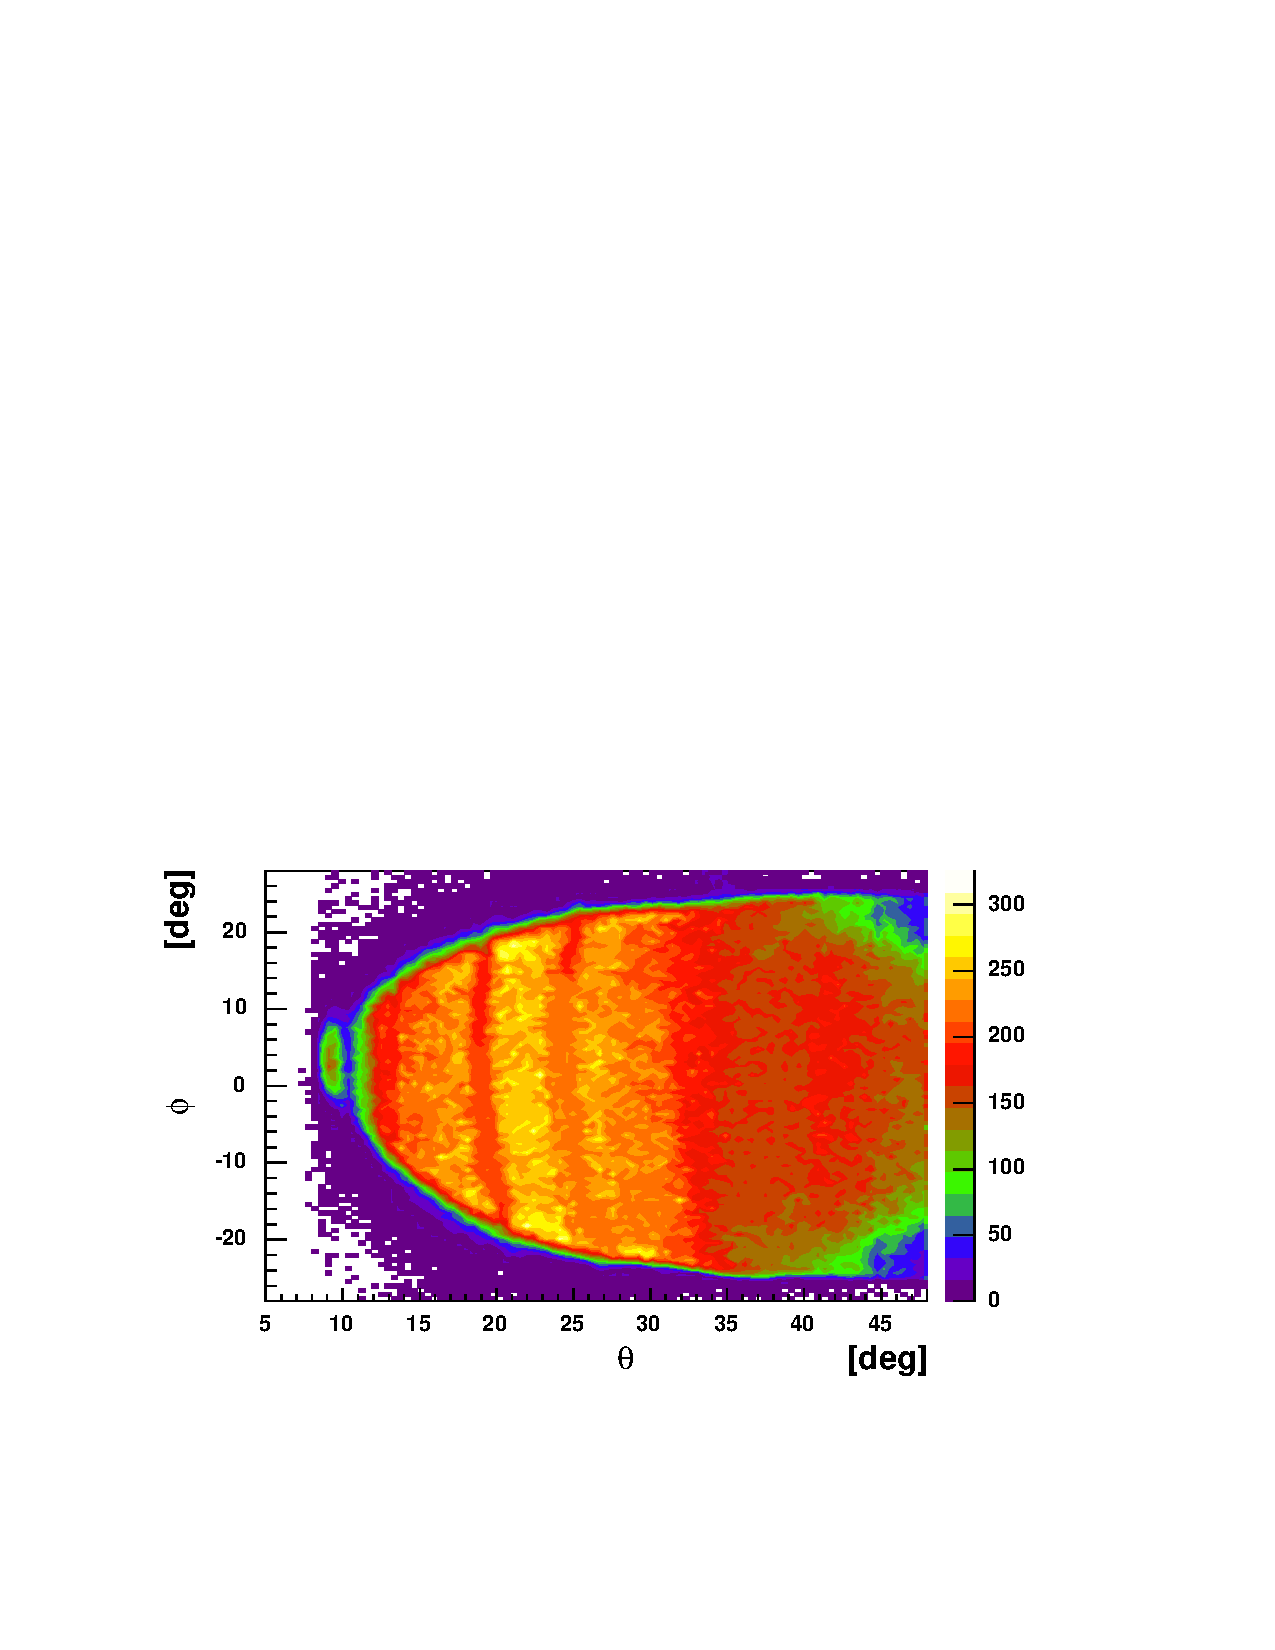
\includegraphics[width = 13cm, bb=40 120 520 420]{img/proton_tph}
  \caption[$\phi$ versus $\theta$ for sector 5 protons]
           { $\phi$ versus $\theta$ for sector 5. The momentum ranges from $0.9$
	              to $1.6$ GeV. The distribution is $\phi$-asymmetric.
                      Depletions along $\phi$ similar to the electron case are visible. }
 \label{fig:proton_tph}
 \end{center}
\end{figure}

In order to evaluate $\phi$ boundaries the momentum has been divided into momentum and $\theta$ bins,
and the distributions were fitted with the tent function shown in appendix \ref{sec:tent_function}.
An example of such fit is shown in Fig.~\ref{fig:tent_fit_s5}.

\begin{figure}[tbp]
 \begin{center}
 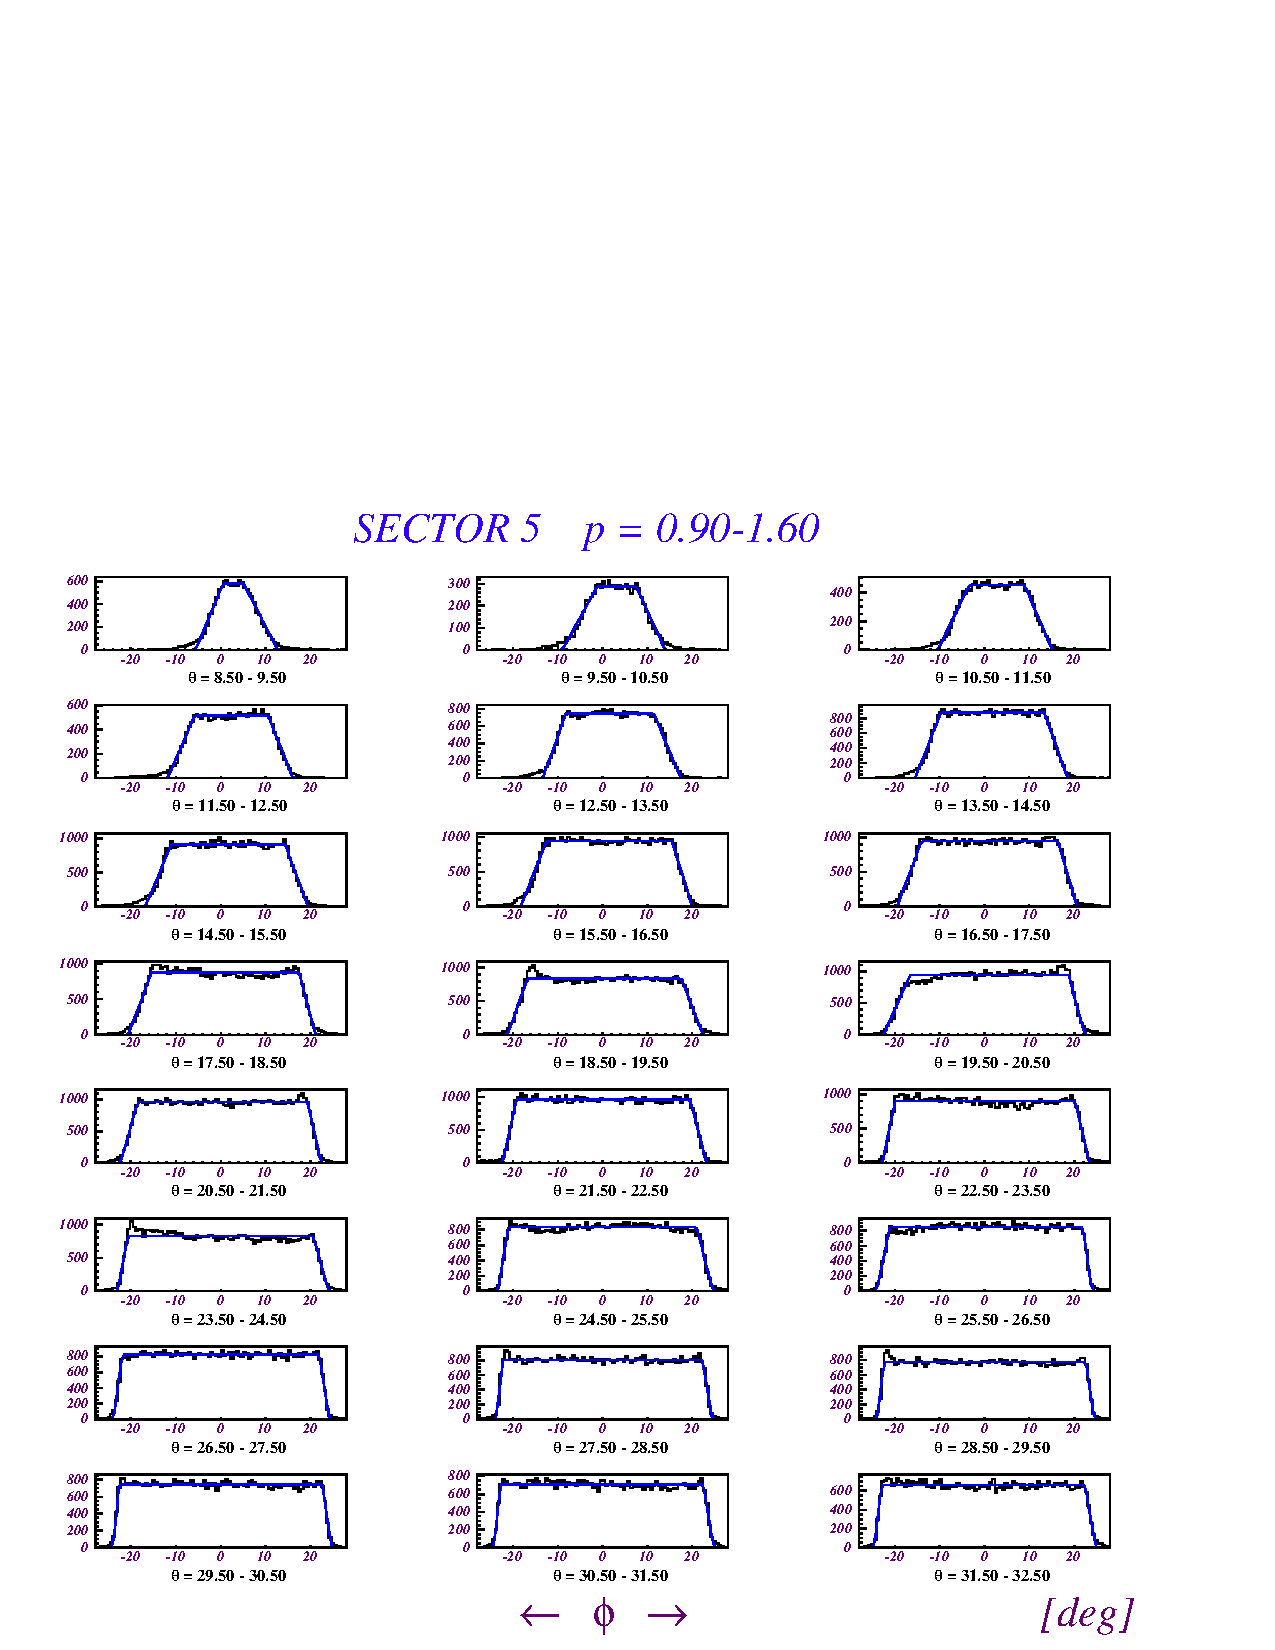
\includegraphics[width = 16cm, bb=0 0 560 560]{img/traped_fit_s5}
  \caption[Trapezoid fit for sector 5]
          { Trapezoid fit for sector 5. The limits of the flat $\phi$ region of each fit
                     will determine the fiducial cut.}
 \label{fig:traped_fit_s5}
 \end{center}
\end{figure}

The parameters are fitted as a function
of $\theta$ with a fourth order polynomial:
$$
\begin{array}{c}
 \phi_{MIN} = a_0 + a_1\theta + a_2\theta^2 + a_3\theta^3 + a_4\theta^4 \\
 \phi_{MAX} = b_0 + b_1\theta + b_2\theta^2 + b_3\theta^3 + b_4\theta^4 \\
\end{array}
$$

Fig.~\ref{fig:traped_fit_result_s5} shows the calculated $\phi_{MIN}$ and $\phi_{MAX}$  and the resulting fit
for sector 5 and momentum range $0.9$ to $1.6$ GeV.

\begin{figure}[h]
 \begin{center}
 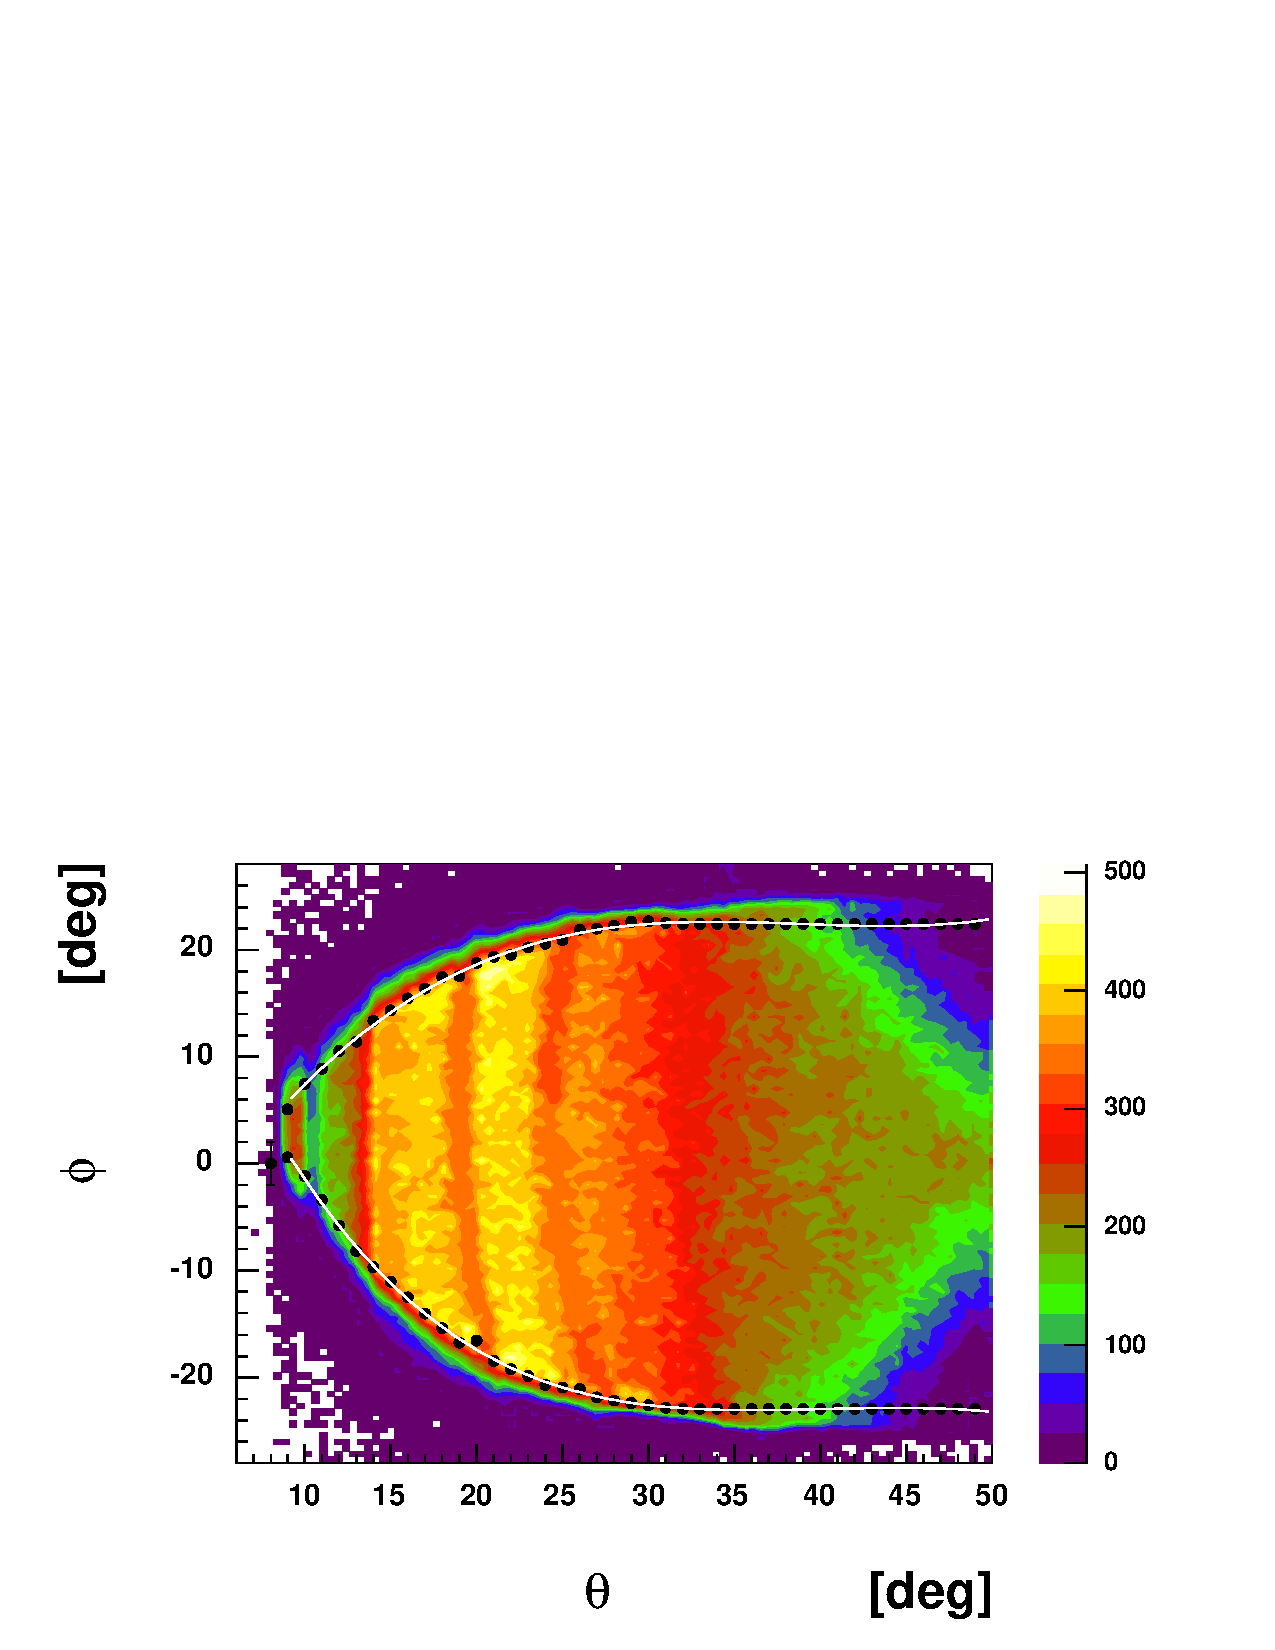
\includegraphics[width = 13cm, bb=0 0 580 430]{img/traped_fit_result_s5}
  \caption[Result of the trapezoid fit]
          { Result of the trapezoid fit for sector 5. The proton momentum ranges from $0.9$
	             to $1.6$ GeV.
	             The black points are the parameters $p_1$ (negative $\phi$) and $p_2$ (positive $\phi$)
                     for each $\theta$ slice considered as shown in Fig.~\ref{fig:traped_fit_s5}.
		     The white line is a fourth order polynomial fit to the black points.}
 \label{fig:traped_fit_result_s5}
 \end{center}
\end{figure}

\subsection{ $\theta$ versus momentum cuts}
Sector 2, 3, 5 and 6 present holes and depletions which are taken care of with the
cuts shown on Fig.~\ref{fig:proton_tp} where $\theta$ is plotted against the momentum $p$.

\begin{figure}[h]
 \begin{center}
 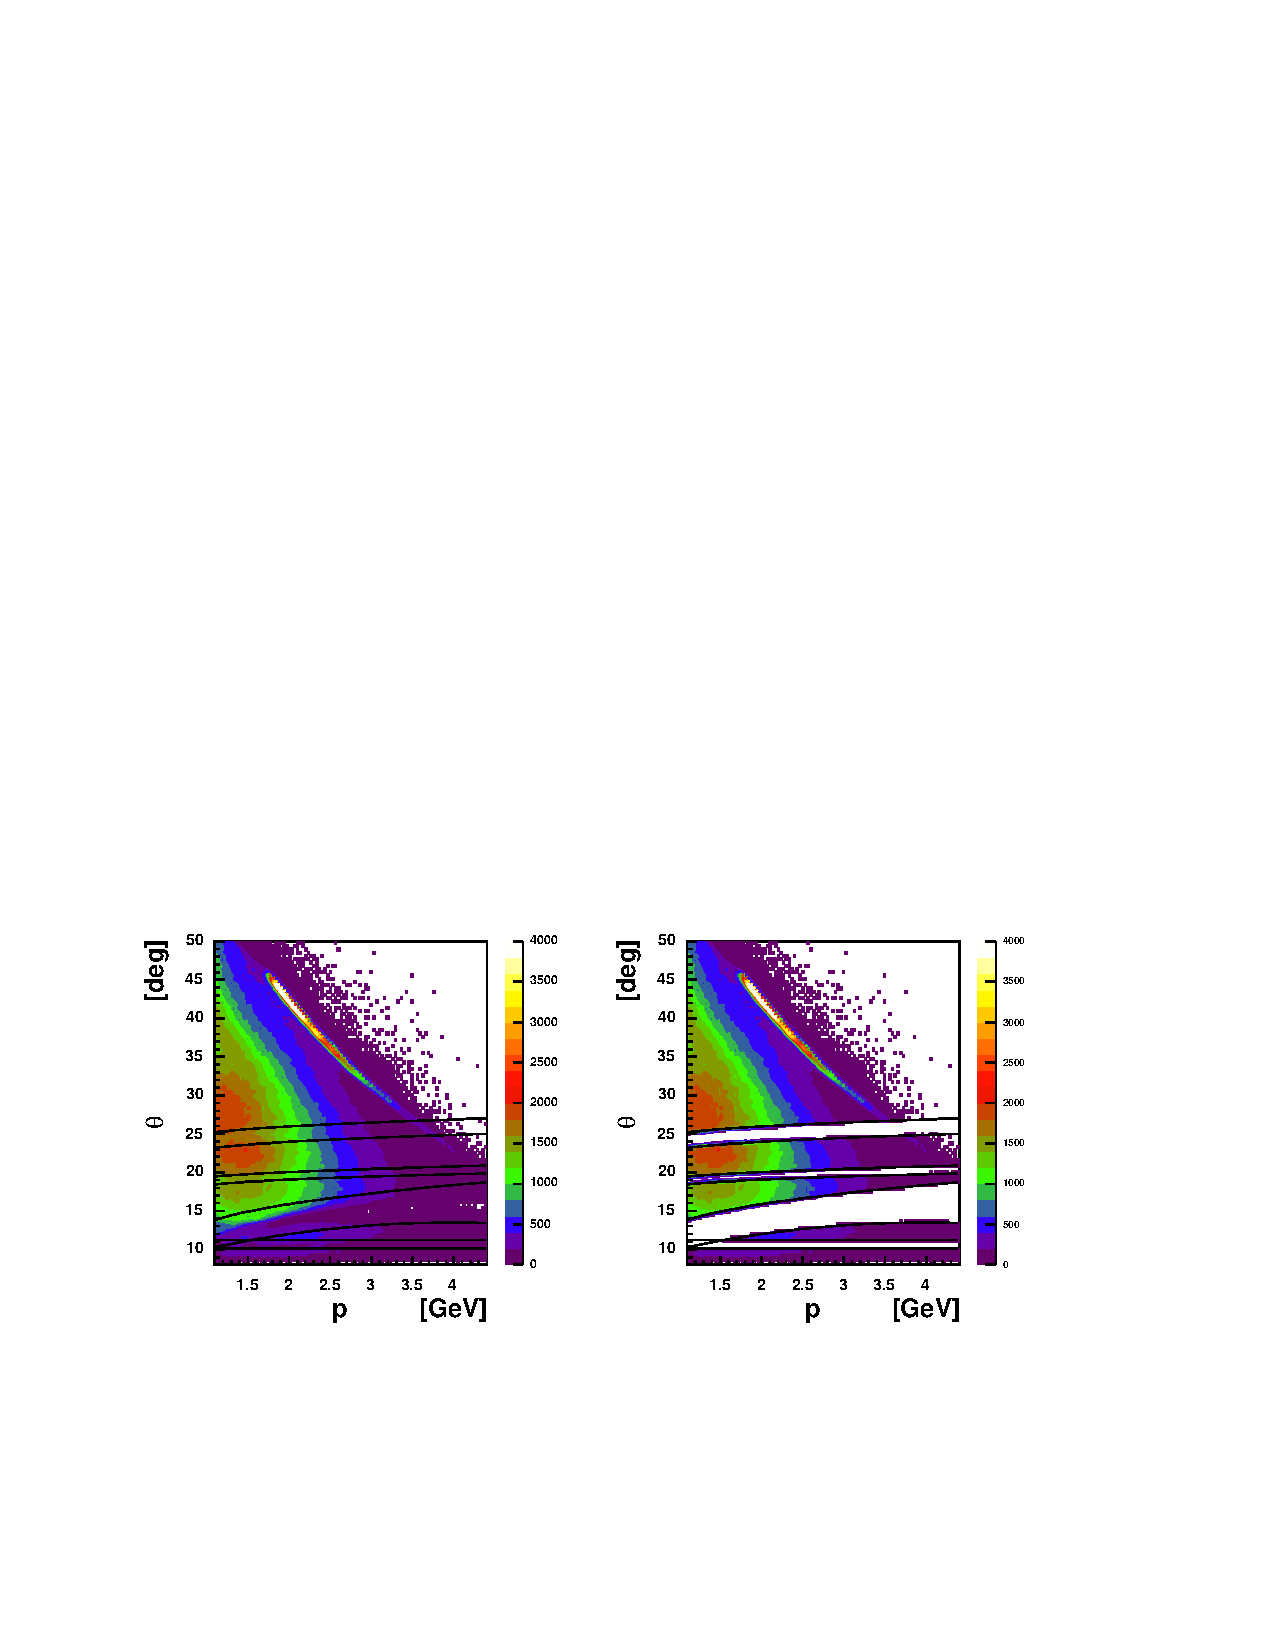
\includegraphics[width = 15cm, bb=20 140 520 380]{img/proton_tp}
  \caption[$\theta$ versus $p$ for protons sector 5]
          { $\theta$ versus $p$ for protons sector 5. A depletion is clearly visible and cut out.}
 \label{fig:proton_tp}
 \end{center}
\end{figure}


The effect of the fiducial cut on sector 5 is shown in Fig.~\ref{fig:fid_p_sector5_result}.

\begin{figure}[h]
 \begin{center}
 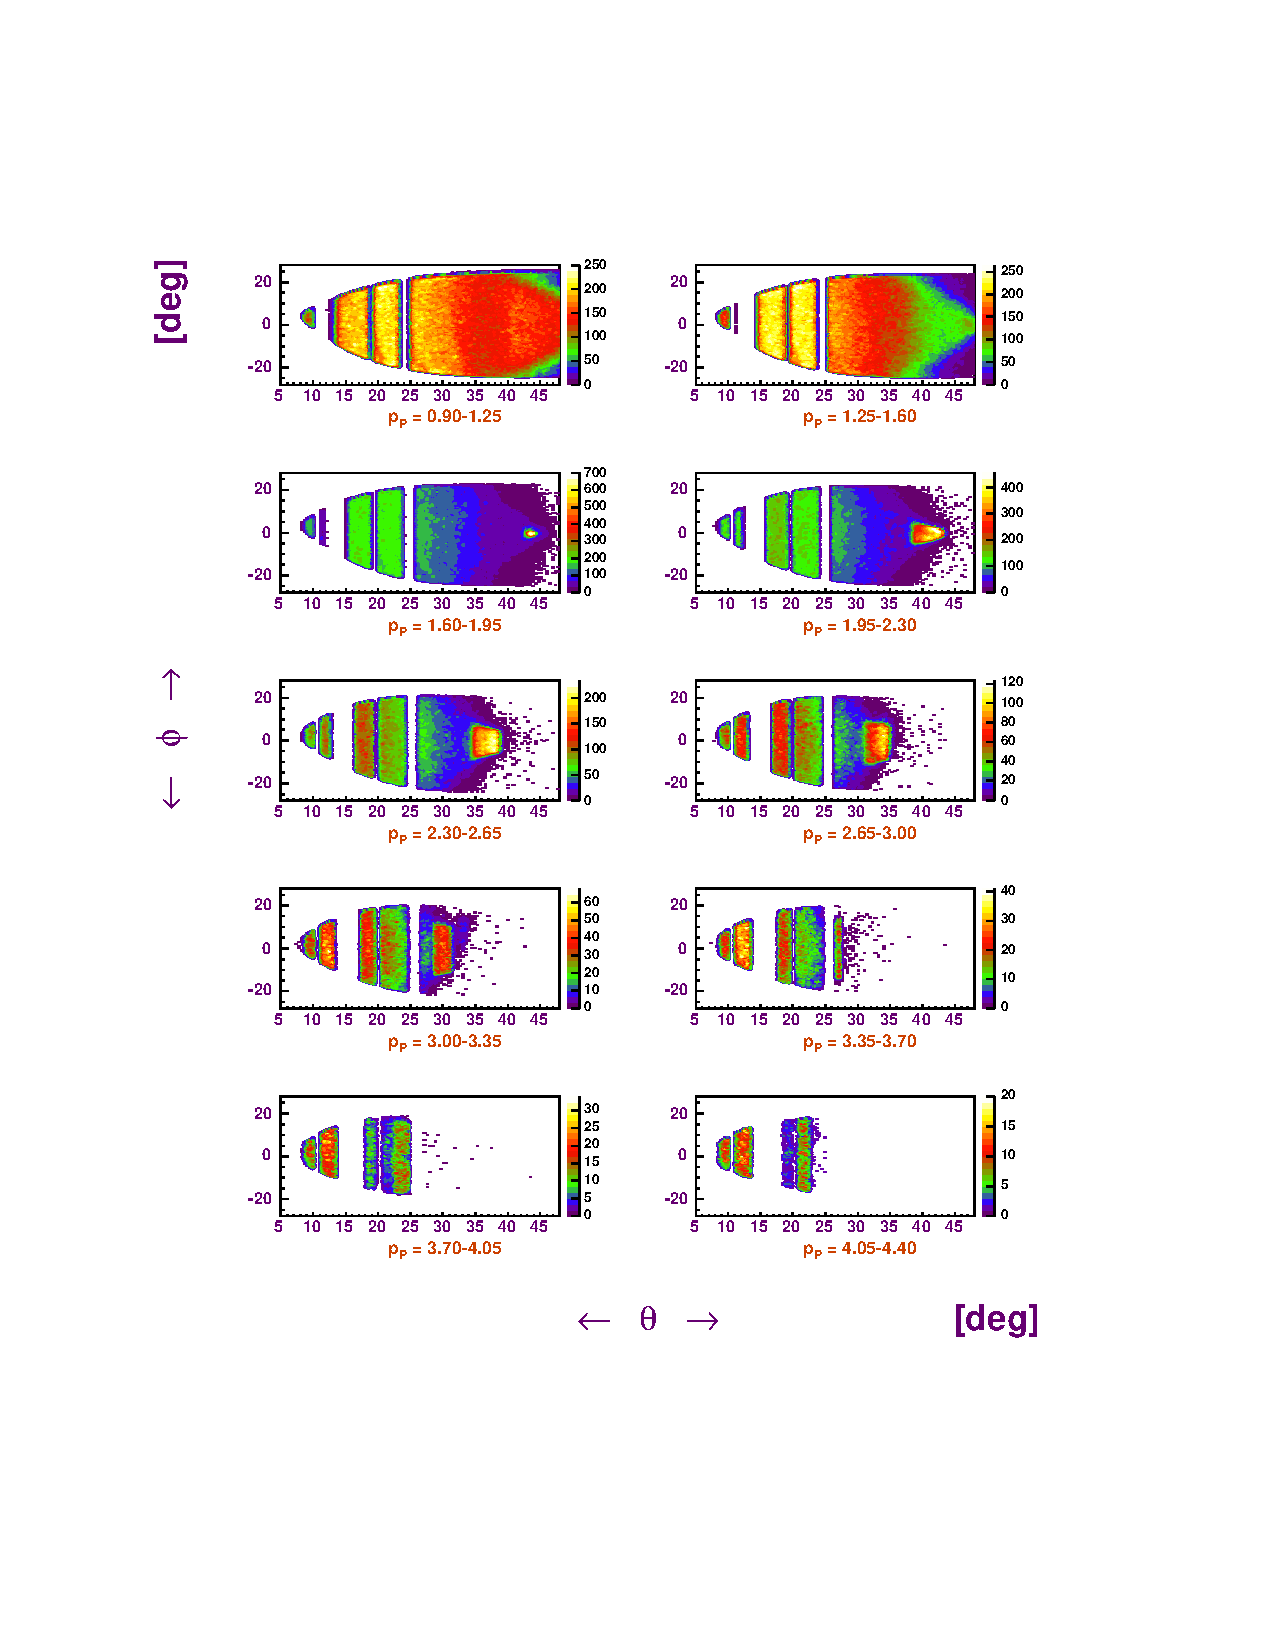
\includegraphics[width = 14cm, bb=60 140 500 660]{img/fid_p_sector5_result}
  \caption[Sector 5 $\phi$ versus $\theta$ after fiducial cut]
          { Sector 5 $\phi$ versus $\theta$ after fiducial cut. The empty bands
	             in this sector are unfortunate because the forward ones occur
		     where many protons of interest to us are expected. }
 \label{fig:fid_p_sector5_result}
 \end{center}
\end{figure}




\subsection{Cuts on detectors coordinates}

The X vs Y distributions of the proton tracks in the DCs and the SC planes in sector 1 are shown in Fig.~\ref{fig:xy_all_planes_s1}.
This section describes the algorithm used to select thigh occupancy regions edges.

\begin{figure}[h]
    \centering
    \includegraphics[width=0.48\textwidth ]{img/plane-DC1_intsector-1}
    \includegraphics[width=0.48\textwidth ]{img/plane-DC2_intsector-1}
    \includegraphics[width=0.48\textwidth ]{img/plane-DC3_intsector-1}
    \includegraphics[width=0.48\textwidth ]{img/plane-SC_intsector-1}
    \caption{The X vs Y distribution of the tracks in the drift chambers and the time
    of flight detector plane (SC) for sector 1. The edges selection algoritm described in the text resulted
    in the black lines, which are the fit of the Y distributions for each X bin.}
    \label{fig:xy_all_planes_s1}
\end{figure}

\clearpage\newpage

In each sector and each plane, 12 bins in X are defined; in each bin, the Y distribution
is fitted with a ``tent'' function $t(y)$ (defined in appendix~\ref{sec:p_tent_function} ) to select the high efficiency edges.
An example of such fit is show in Fig.~\ref{fig:y_slices_s1} for sector 1 in the DC3 plane, for 4 bins in X.
The fit cleanly identifies the steep rises and falls of the distributions and the relatively flat regions in between.


\begin{figure}[h]
    \centering
    \includegraphics[width=0.48\textwidth ]{img/slice-05_sector-1_plane-DC1}
    \includegraphics[width=0.48\textwidth ]{img/slice-06_sector-1_plane-DC1}
    \includegraphics[width=0.48\textwidth ]{img/slice-07_sector-1_plane-DC1}
    \includegraphics[width=0.48\textwidth ]{img/slice-08_sector-1_plane-DC1}
    \caption{Y distribution for 4 X bins in the DC3 plane for sector 1. The black lines are the tent
    fit of the Y distributions. The result of the first is the two points of intersection between the straight
    lines (steep rise) and the parabole fit (flat region). The two points are then plotted in the XY plane and
    fitted with a parabola, see for example Fig.~\ref{fig:xy_all_planes_s1} or Fig.~\ref{fig:xy_dc12_s5}.}
    \label{fig:y_slices_s1}
\end{figure}

The results of the tent fit are the two points of intersection between the straight lines (steep rise) and the
parabola fit (flat region). The two points are then plotted in the XY plane for all the X bins and fitted with
a parabola, see for example Fig.~\ref{fig:xy_all_planes_s1} or Fig.~\ref{fig:xy_dc12_s5}.

This procedure results in a fiducial cut function for each plane and each sector.


\newpage

\subsubsection{Detectors inefficiencies}
The detector coordinates plots allow to correlate hardware inefficiencies with depletions in the XY distributions.
For example, in the DC planes, where neighboring group of wires are powered by the same HV supply and
axial and stereo wires are tilted by $6^0$ with respect to each other, the inefficiencies
will appear as:

\begin{itemize}
    \item Axial wires: horizontal bands in the XY distributions
    \item Stereo wires: $6^0$ tilted bands in the XY distributions
\end{itemize}

Two examples of such hardware problems in sector 2 are summarized in Fig.~\ref{fig:xy_dc12_s5}.
These regions are removed with dedicated cuts represented by straight lines in the XY plane,
horizontal for the axial wires and $6^0$ tilted for the stereo wires. Notice: these are the
same cuts used for the electrons.

\begin{figure}[ht]
    \centering
    \includegraphics[width=0.48\textwidth ]{img/plane-DC2_intsector-5}
    \includegraphics[width=0.48\textwidth ]{img/plane-DC1_intsector-5}
    \caption{The X vs Y distribution of the proton tracks intersection wiht the DC2 (left)
        and DC1 (right) planes in sector 5. The left distributions shows one depletion for the stereo wires,
        while the right distribution shows two depletions for the axial wires.}
    \label{fig:xy_dc12_s5}
\end{figure}

\subsubsection{Comparison with the traditional cuts}

The effect of the fiducial and inefficiencies cuts are compared with the traditional $\phi, \theta, p$ cuts.
The comparison highlights the advantages of the new approach:

\begin{itemize}
    \item identify the real edge effects in the detector
    \item hardware problems are represented by straight lines in the XY plane
    \item no momentum dependence of the cuts
\end{itemize}

This comparison is shown as an example for sector 2 and a momentum bin in Fig.~\ref{fig:PnPvsTmom-2.4_sector-2_plot-phiVsTheta}.
The before and after $\phi$ vs $\theta$ distributions in sector 2 for all the momentum bin are shown in Fig.~\ref{fig:phiTheta-before_sector-5}
and~\ref{fig:phiTheta-after_sector-5} respectively.

The complete set of plots is available at~\ref{bib:pi0_resonance_fiducial_proton}.

\begin{figure}[ht]
    \centering
    \includegraphics[width=0.98\textwidth ]{img/PnPvsTmom-2.4_sector-2_plot-phiVsTheta}
    \caption{Comparison between the traditional cuts (function of $\phi, \theta, p$) and the new cuts on the XY detector coordinates.
    Top left:  $\phi$ vs $\theta$ before any cuts. Top right:  $\phi$ vs $\theta$ after the XY cuts cuts. The traditional cuts superimposed
    and shown with black lines. Notice that the traditional cuts would remove events at very small $\theta$ and large $\phi$, due to its functional form.
    Bottom left: DC1 plane after the fidu XY cuts. Bottm right: DC2 plane after the fidu XY cuts.
    Notice how the DC1 axial wires depletion is reflected in the DC2 plane. This reflection moves depending on the momentum bin and would be hard to model
    using the traditional cuts.}
    \label{fig:PnPvsTmom-2.4_sector-2_plot-phiVsTheta}
\end{figure}




\begin{figure}[ht]
    \centering
    \includegraphics[width=0.98\textwidth ]{img/phiTheta-before_sector-2}
    \caption{$\phi$ vs $\theta$ distributions in sector 5 for all the momentum bin before the XY fiducial cuts.}
    \label{fig:phiTheta-before_sector-5}
\end{figure}

\begin{figure}[ht]
    \centering
    \includegraphics[width=0.98\textwidth ]{img/phiTheta-after_sector-2}
    \caption{$\phi$ vs $\theta$ distributions in sector 5 for all the momentum bin after the XY fiducial cuts.}
    \label{fig:phiTheta-after_sector-5}
\end{figure}




